\chapter{Leitungstheorie und Fertigung}
In dieser Arbeit werden verschiedene Leiterplatten gefertigt. Eine solche Leiterplatte wird auch  PCB\footnote{\textbf{P}rinted \textbf{C}ircuit \textbf{B}oard} genannt. Diese Form der Leiterplattenherstellung ist bei Frequenzen von unter \SI{100}{\giga\hertz} üblich. Eine Leiterplatte ist aus verschiedenen Lagen aufgebaut. Entscheidend hierfür sind gewählte Dielektrika sowie die Materialdicken und die Lagenverteilung. Durch Ätzen, Bestrahlen und Kleben werden somit gewünschte Strukturen aufgebaut.  \\
Teil von PCBs sind immer planare Steifenleitungen. Die Signalführung auf planaren Steifenleitungen ist nur in seltenen Fällen exakt mathematisch berechenbar. Weiterhin wird ein Modell zur Berechnung einer Mikrostreifenleitung vorgestellt.
\section{Mikrostreifenleitung}
\begin{figure}[tp]
  \centering
  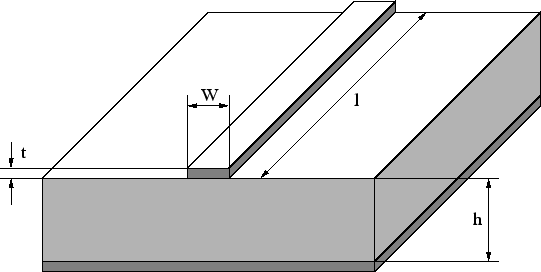
\includegraphics[scale=0.5]{gfx/MSL.png}
  \caption{Aufbau einer Mikrostreifenleitung\cite{MSL}}
  \label{fig:MSL}
\end{figure}
Eine Mikrostreifenleitung , dargestellt in Bild \ref{fig:MSL}, besteht aus einer leitenden Metallschicht auf der Oberseite eines Substrats. Unter diesem Substrat befindet sich ebenfalls eine leitende Metallschicht, die Massefläche\footnote{Auch Ground-Plane, die Bezugsfläche für das Potenzial}. Dabei sind die Substrat-Höhe $h$, die Metallbreite $W$, die Metallhöhe $t$ sowie die Dielektrizitätszahl $\epsilon_{r}$ des Substrats die charakteristischen Größen der Mikrostreifenleitung. Es muss für verschiedene Frequenzen von Signalen die Geometrie der Mikrostreifenleitung angepasst werden\cite{TransmissionLineDesignHandbook}. Da sich die elektromagnetische Welle überwiegend innerhalb des Substrats befindet, ist die effektive Dielektrizitätszahl $\epsilon_{r,eff}$ eine Möglichkeit die Feldverteilung mathematisch einfach darzustellen. Dabei ändert sich die ursprüngliche Geometrie der Mikrostreifenleitung mit Hilfe von $\epsilon_{r,eff}$ und der effektiven Leiterbahnbreite $W_{eff}$. Für $\epsilon_{r,eff}$ gilt dabei für $w/h < 1 $
\begin{align}
\epsilon_{r,eff} = \frac{\left( \epsilon_{r}+1 \right)}{2} + \frac{\left( \epsilon_{r}-1 \right)}{2} \cdot \left[ \left( 1 + \frac{10h}{W}\right)^{-0.5}+ 0.04 \left( 1.0 - \frac{w}{h}\right)^2\right]
\end{align}
sowie für $ w/h > 1$
\begin{align}
\epsilon_{r,eff} = \frac{\left( \epsilon_{r}+1 \right)}{2} + \frac{\left( \epsilon_{r}-1 \right)}{2} \cdot \left( 1 + \frac{10h}{W}\right)^{-0.5}.
\end{align}



\subsection{Differentielle Signalübertragung}
Eine differentielle Leitung besteht aus zwei Leiterbahnen. Auf jeder Leiterbahn ist ein Signal, welche zueinander komplementär sind, also $180^\circ $  Phasenverschiebung zueinander haben. Verglichen mit herkömmlichen Leitungen haben differentielle Leitungen einige Vorteile 
\begin{description}
\item Unterschiede im Bezugspotenzial zwischen Systemkomponenten haben kaum Einfluss auf Logiklevel.
\item Dämpfung auf einer Leiterbahn ist kompensierbar. Nach \cite{DifferentialSignalLine} lässt sich bis zu 24dB Dämpfung kompensieren.
\item Höhere Datenraten sind möglich. Dabei ist nach \cite{DifferentialSignalLine} bis zu  eine Datenrate von 10Gb/S möglich.
\end{description}
wobei stets mehr Leitungen nötig sind, um die gleiche Anzahl Signale zu führen, wenn pro Signal je eine Leitung verwendet wird. 
\begin{figure}[tbp]
  \centering
  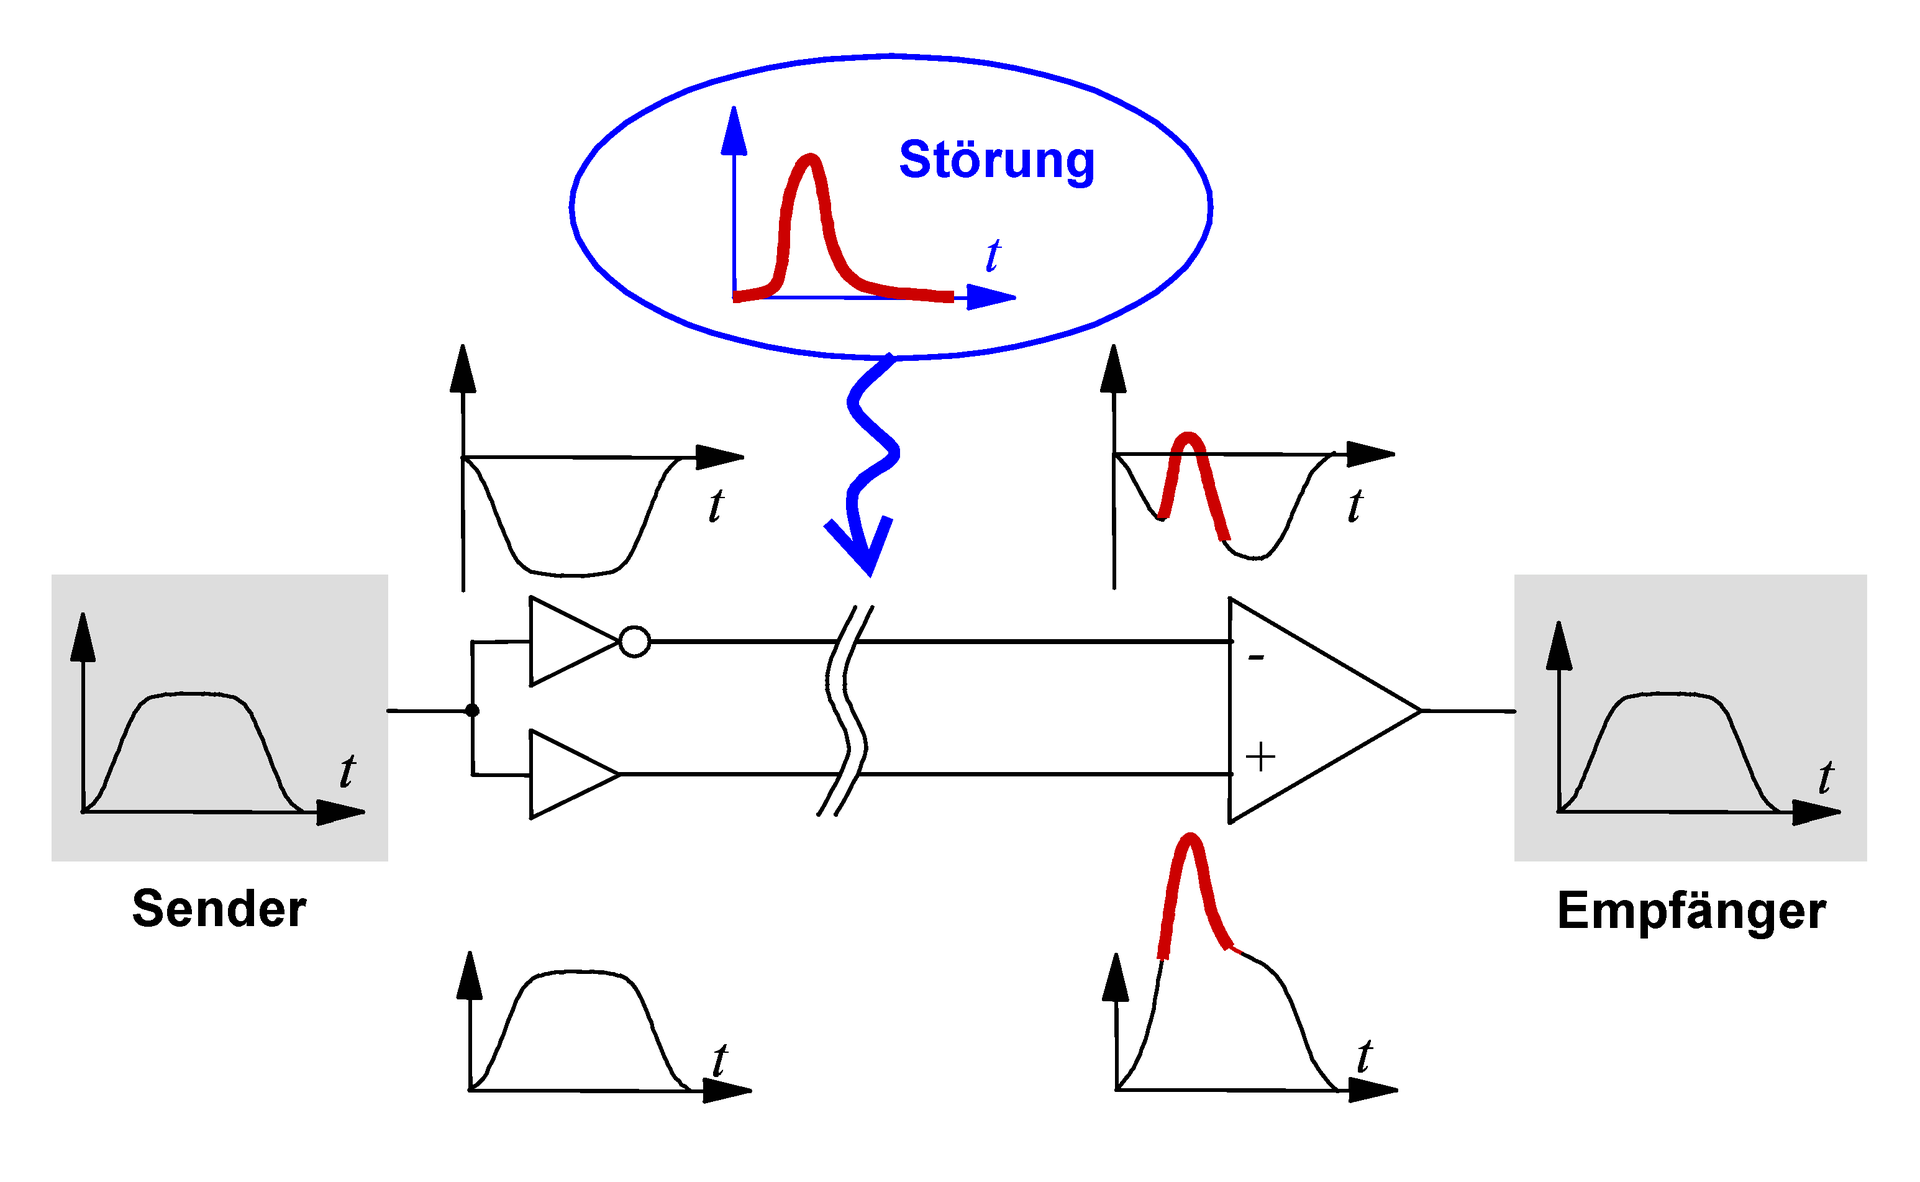
\includegraphics[scale=1.5]{gfx/DiffSignalUebertragung.png}
  \caption{Einfluss einer Störung auf Differentielle Signalübertragung\cite{DiffSig}}
  \label{fig:DiffSig}
\end{figure}
In \ref{fig:DiffSig} ist eine differentielle Leitung dargestellt. Auf beide Signale wirkt dabei die gleiche Störung. Ist auf \ref{fig:DiffSig} die invertierte Leitung $s_{1}$ mit dem dazugehörigen Signal $-s(t)$ sowie die nicht invertierende Leitung $s_{2}$ mit $s(t)$ jeweils die Störung $e(t)$ addiert, ergibt sich durch die Differenz der am Operationsverstärker anliegenden Signale $f$ und $g$ mit 
\begin{align}
f(t) &= -s(t) + e(t) \\
g(t) &=  s(t) + e(t)
\end{align}
als Ausgang $s_{Res}(t)$ von
\begin{align}
s_{Res}(t) = g(t) - f(t)= 2\cdot s(t).
\end{align}
Dabei wird das SNR um 6dB verbessert.\\
Für die Leitungsanpassung der differentiellen Leitung muss die Impedanz der differentiellen Leitung $Z_{Diff}$ berechnet werden. Diese ergibt sich zu 
\begin{equation}
Z_{Diff} = 2Z_{0} \left( 1- 0.48e^{\left(-0.96\frac{s}{h} \right)} \right).
\end{equation}
Hier ist $s$ der Abstand zwischen den beiden einzelnen Leitungen. Häufig soll $Z_{Diff}$ = \SI{100}{\ohm} ergeben um optimal auf angepasst zu sein. Demnach kann dies bei entweder über $Z_{0}$ oder über $s$ eingestellt werden.Die jeweiligen Leitungslängen müssen gleich lang sein. Andernfalls ergibt sich ein Phasenunterschied der eine eindeutige Filterung verhindert, da dadurch gegebenenfalls Störungen zu unterschiedlichen Zeitpunkten anliegen. Je nach Frequenz des Signals verhindern bereits kleine Abweichungen die eindeutige Rekonstruktion des ursprünglichen Signals. Diese Abweichungen lassen sich leicht mit \ref{eq:fzulambda} berechnen. Ist die Toleranz der Leitungslänge etwa \SI{1}{\percent} so ist der zulässige Leitungslängenunterschied $\Delta l_{max}$ bei einer Frequenz von \SI{10}{\mega\hertz} $\Delta l_{max} = $ \SI{30}{\centi\meter}, bei einer Frequenz von \SI{2.4}{\giga\hertz} allerdings $\Delta l_{max} =$ \SI{1.25}{\milli\meter}. Der  Leitungslängenunterschied innerhalb einer Toleranz nimmt mit zunehmender Frequenz ab. Je nach Anwendung kann auch ein Bauteil-Takt die Toleranz vorgeben. Zusätzlich muss um eine Störung nur symmetrisch auf beide Leitungen zu erhalten der Leitungsabstand zueinander gering und konstant sein. Je nach Leitungsart ist dies allerdings auf Grund von Feldverteilungen nicht immer möglich.

\section{Lagenaufbau und Substrate}

Es werden Lagen entweder aus Kupfer oder aus einem Dielektrikum aufgebaut. Dabei dienen Kupferlagen insbesondere zur Abschirmung als Masse-Fläche oder Power/Ground-Lage. Zusätzlich sind Kupferlagen für die thermische Fluktuation, also zur Kühlung, geeignet. Besonders wichtig ist es, keine Inseln von Kupferlagen zu erzeugen. Diese Inseln haben kein definiertes Potenzial und verursachen potenziell Störungen. \\
Lagen aus einem Dielektrikum werden als Träger für Leiterbahnen verwendet. Dabei ist insbesondere die Dielektrizitätszahl entscheidend.\\
Es werden in dieser Arbeit drei verschiedene Substrate verwendet. Diese sind in Tabelle \ref{tab:FR4} dargestellt.
\begin{table}[tbp]
  \centering
  \begin{tabular}{lccr}
    Substratmaterial  & FR4 & Rogers4003 &Rogers3003\\
    \hline
    Dielektrizitätszahl $\epsilon_{r}$ & 5.0 & 3.38 & 3.0 \\
    Verlustfaktor $\tan \left( \delta \right)$ & 0.02 & 0.0021& 0.001 \\
    Oberflächenwiderstand & $\geq$\SI{10}{\kilo\ohm}& $\geq$\SI{4.2}{\giga\ohm} & $\geq$\SI{1}{\mega\ohm} \\
    Durchgangswiderstand & $\geq$\SI{10}{\kilo\ohm}&$\geq$\SI{17}{\giga\ohm}& $\geq$\SI{1}{\mega\ohm}\\
  \end{tabular}
  \caption{Materialparameter verwendeter Substrate}
  \label{tab:FR4}
\end{table}
FR4 ist ein gebräuchliches Substrat Material aus Epoxydharz-Glasfaser-Gewebe in der PCB-Herstellung. Die Eigenschaften von FR4 sind in Tabelle \ref{tab:FR4} dargestellt, wobei insbesondere der niedrige Preis und die einfache Verarbeitung, d.h. das Substrat ist fest und demnach nicht leicht verformbar, im Vergleich zu anderen Substraten von Vorteil ist.
\\
Ein Lagenwechsel, auch VIA, besteht aus einem PAD und einer zugehörigen Bohrung. Dabei sollen VIAs sowohl elektrisch als auch thermisch verbinden. Es gilt verschiedene Typen ,Bild \ref{fig:VIA}, von VIAs zu unterscheiden.
\begin{figure}[tbp]
  \centering
  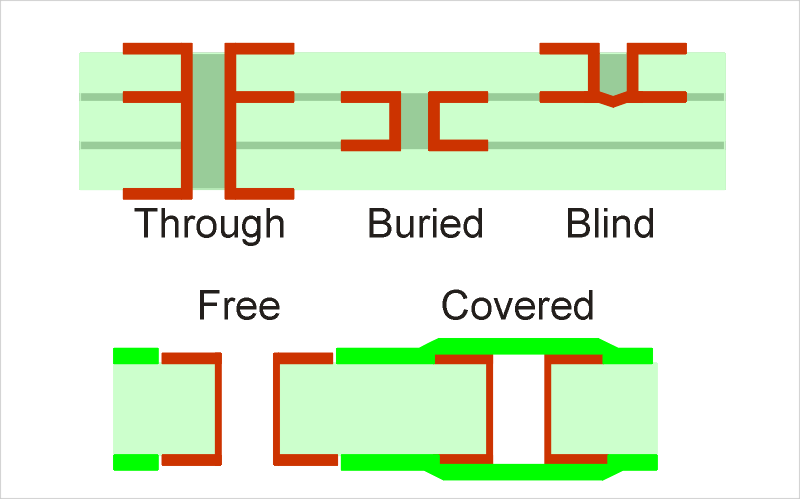
\includegraphics[scale=0.5]{gfx/VIA.png}
  \caption{Verschiedene VIA\cite{VIA}}
  \label{fig:VIA}
\end{figure}
Dabei ist insbesondere das Through VIA weiterhin von Bedeutung. Durch dieses VIA lässt sich besonders gut thermische Leitfähigkeit sicherstellen und zusätzlich sind Through VIAs hervorragend als Messpunkte für die Inbetriebnahme von PCBs geeignet. \\
Wichtig sind die bei der Fertigung auftretenden Herstellungstoleranzen. Die Dicke einzelner Lagen kann sich um bis zu \SI{20}{\percent} verändern. Ebenfalls können sich einzelne Lagen zueinander verformen. Dabei sind besonders Innenlagen betroffen. Auch Bohr- oder Ätzungenauigkeiten sind zu berücksichtigen. Dabei sollten stets \SI{20}{\micro\meter} Toleranz bedacht werden. Demnach muss bei der Dimensionierung einer Komponente beachtet werden, dass die Größe um $\pm \SI{20}{\micro\meter}$ variiert. Dies tritt insbesondere bei Abständen von Komponenten zueinander auf. Jeder Abstand sollte demnach mindestens doppelt so groß sein wie die einfache Toleranz.
\subsection{Auslegung von Signalleitungen}
Signale oder Spannungen werden auf Kupfer geleitet. Dabei werden Spannungen eher über Ebenen geführt als über Leitungen mit konstante Breite. Dies resultiert aus der umgekehrten Proportionalität der Leitungsbreite zum Leitungswiderstand. Ein geringer Widerstand sorgt dabei für geringe Spannungsverluste auf dem PCB.\\
Signale werden entweder Single-Ended oder Differentiell geführt. Besonders digitale Signale sind dabei Single-Ended. Das eigene Zwischenfrequenzsignal wird auf dem PCB Differentiell geführt und erst mit der letzten Systemkomponente Single-Ended umgewandelt.\\
Die zu erwartende Bandbreite sind bis zu \SI{20}{\mega\hertz}. Bei diesen Frequenzen sind geringe Längenunterschiede in der differentielle Leitung tolerierbar, da bei angenommenen \SI{20}{\mega\hertz} ein Längenunterschied von \SI{8}{c\meter}, der gesamten Länge des PCB, nur ein relativer Fehler von 0.01875 oder von 10.6 Grad Phase auftritt. Da ein Fehler dieser Größenordnung bedeutet, dass eine Leitung über das gesamte PCB führt und die andere nicht existiert, kann der Fehler durch Längenunterschiede als klein genug angenommen werden um nicht weiter berücksichtigt zu werden.\\
Entsprechende Signalleitungen sind stets von Through-Vias umgeben. Diese sorgen für einheitliche Referenzpotenziale um die Leitungen herum. Zusätzlich sind Knicke von mehr als \SI{45}{\degree} zu vermeiden. Bei stärkerem Knick ändert sich abrupt die Impedanz der Leitung und verursacht demnach Reflexionen, die vermieden werden müssen. Theoretisch wären Leiterbahnbögen die beste Wahl, allerdings sind diese in der Herstellung deutlich aufwändiger im Vergleich zu \SI{45}{\degree} Winkeln und bringen dabei keine wesentliche Fortschritte in den betrachteten Frequenzen.\\